\chapter{Resultados}
Nesse capítulo os resultados das diferentes soluções propostas no trabalho são apresentados. Primeiramente introduzem-se as medidas de avaliação que serão utilizadas. Em seguida compara-se as etapas de classificação do método tradicional e híbrido, cujo processo de seleção de candidatos é idêntico, portanto a diferença em desempenho se dá apenas no estágio de classificação. Por fim avalia-se o desempenho do sistema completo das diferentes soluções apresentadas.

\section{Medidas de avaliação}
Para avaliar o desempenho das diferentes soluções apresentadas nesse trabalho se faz necessário a utilização de medidas que permitam comparar os resultados objetivamente e indicar facilmente os aspectos positivos e negativos relevantes de cada método. Nesse trabalho tratamos de classificação binária, em que amostras são positivas (representando cabeças e também indicadas por 1) ou negativas (representando não-cabeças e também indicadas por 0). 

Em geral, num problema de classificação o indicador mais comum é a acurácia (\textit{accuracy}), definida \cite{evaluationMetrics} como a razão das classificações corretas pelo total de classificações. É fundamental notar, entretanto, que essa medida sozinha não é suficiente para avaliar um classificador, especialmente se o dataset for desbalanceado. Por exemplo, ao considerar um dataset com duas amostras negativas entre 20 e utilizar um classificador trivial que classifica qualquer amostra como sendo positiva, obtem-se uma acurácia de 90\%, demonstrando o problema dessa métrica.

Uma maneira compacta de representar o desempenho de um classificador é a \textbf{matriz de confusão} \cite{evaluationMetrics}. Para uma classificação binária é uma matriz 2x2 em que a primeira linha indica as amostras negativas e a segunda as amostras positivas. De forma semelhante, a primeira coluna indica amostras que foram classificadas como negativas e a segunda que foram classificadas como positivas. Combinando-se essas linhas e colunas, obtém-se o número de verdadeiros negativos TN, falsos positivos FP, falsos negativos FN e verdadeiros positivos TP, respectivamente. Essa estrutura supera os problemas da acurácia pois fornece a distribuição de acertos e erros de classificação. Adota-se a descrição dos valores em percentuais relativos ao conjunto de análise.

\begin{table}[h]
\centering
\caption{Matriz de confusão}
\label{tab:matriz-confusão}
\begin{tabular}{ll|l|l|}
\cline{3-4}
                                            &   & \multicolumn{2}{l|}{Classificado} \\ \cline{3-4} 
                                            &   & 0               & 1               \\ \hline
\multicolumn{1}{|l|}{\multirow{2}{*}{Real}} & 0 & \text{TN}              & \text{FP}              \\ \cline{2-4} 
\multicolumn{1}{|l|}{}                      & 1 & \text{FN}              & \text{TP}              \\ \hline
\end{tabular}
\end{table}

Outro aspecto a destacar na avaliação de classificadores é que não basta avaliar os indicadores apresentados apenas no \textit{dataset}. Embora essas medidas forneçam um limite máximo de desempenho do classificador, não se pode avaliar o desempenho do mesmo em um caso geral. Isso porque o modelo adquire um aspecto de memória das amostras, o que impede a avaliação da generalização do mesmo. Assim, o modelo pode ter se tornado muito específico para o conjunto de dados de treinamento, situação conhecida como \textit{overfitting}. Portanto, para medir o real desempenho do classificador utiliza-se de outro conjunto de dados supervisionados chamado de conjunto de validação -- \textit{validation set}, independente do conjunto de treinamento.

Graficamente pode-se avaliar classificadores através da curva ROC -- \textit{Receiver Operating Characteristic} \cite{evaluationMetrics}, que demonstra como a taxa de verdadeiros positivos -- TVP ($\frac{TP}{FN+TP}$) se relaciona com a taxa de falsos positivos -- TFP ($\frac{FP}{TN+FP}$). Para classificadores discretos, cuja saída é apenas a classe, pode-se representar um ponto no espaço ROC. Já para classificadores com uma saída probabilistica, ao variar o limiar de probabilidade $T$ acima do qual se considera uma amostra como positiva é possível representar diversos pontos, caracterizando uma curva nesse espaço. O melhor classificador indicaria uma taxa de TVP unitária com TFP nula, o que caracteriza uma reta de $(0,1)$ a $(1,1)$ delimitando uma área, AUC (\textit{Area Under Curve}), unitária. Pontos mais próximos do classificador ideal $(0,1)$ são considerados melhores. Portanto, quanto maior a AUC melhor o desempenho do classificador. Além disso, essa curva pode ser utilizada para selecionar o limiar de probabilidade $T$ de forma a atingir uma taxa de TVP especificada ao preço de uma TFP correspondente no caso de saídas probabilísticas.

Um requerimento específico para a aplicação em questão é que a linha de produção se mantenha em funcionamento o maior tempo possível, para tanto deve-se minimizar a quantidade de falsos positivos FP, que significam cabeças incorretamente identificadas que interrompam a produção sem necessidade.

\section{Classificadores}
\label{sec:resultados-classificadores}
O dataset foi gerado a partir de gravações realizadas no ambiente indústrial onde o sistema deverá ser instalado. A câmera foi posicionada num ponto próximo de onde deve ocorrer a sua instalação final. Diversos vídeos foram gravados e posteriormente analisados. Utilizando o algoritmo de detecção de candidatos visto em \ref{sec:tradicional-candidatos}, selecionou-se manualmente em cada quadro quais dos candidatos eram verdadeiramente cabeças. Repetindo esse processo em cada quadro formou-se um dataset, cuja amostra é o recorte do candidato, reduzido de 2459 amostras negativas (não cabeças) e 667 positivas (cabeças). Em seguida extendeu-se esse dataset reduzido para 9894 amostras negativas e 1222 positivas, formando o dataset completo. Criou-se, ainda, um conjunto de validação independente de 2738 amostras negativas e 235 amostras positivas.

\subsection{Método tradicional}
Avaliou-se o resultado das diferentes descritores mencionados em \ref{sec:tradicional-descritores} utilizando um processo de treinamento automático do SVM \cite{scikit-learn}: varreu-se o espaço dos parâmetros $C$ entre $0.0001$ e $0.01$ com passos de $0.001$ e $\sigma$ entre $1$ e $100$ com passos de $5$. Os melhores resultados, selecionados segundo a medida de \textit{precision}, são apresentados na forma de matriz de confusão para cada um dos descritores.

\begin{table}[h]
\cfmat{Grades simples (7x7), dataset completo}{9881}{13}{36}{1186}
\cfmat{Grades simples (7x7), conjunto validação}{2589}{149}{198}{37}
\end{table}

Para o descritor de anéis concêntricos, primeiramente utilizou-se o dataset reduzido para avaliar qual a melhor dimensão do descritor, observando os seguintes resultados.

\begin{table}[h!]
\cfmat{Anéis concêntricos com 8 dimensões, dataset reduzido}{2364}{65}{185}{482}
\cfmat{Anéis concêntricos com 16 dimensões, dataset reduzido}{2385}{44}{111}{556}
\cfmat{Anéis concêntricos com 18 dimensões, dataset reduzido}{2410}{19}{60}{607}
\end{table}

Deseja-se avaliar qual das descrições anteriores demonstra melhor resultado para o problema de detecção de pessoas. Para tanto, treinou-se um classificador SVM para cada uma das descrições utilizando o dataset reduzido. Em seguida avaliou-se o desempenho de cada uma sob o dataset de validação, forçando uma saída probabilística no SVM e assim permitindo traçar uma curva ROC. O resultado se apresenta graficamente sob forma das curvas ROC na figura \ref{fig:roc-rings}.

\begin{figure}[h]
\centering
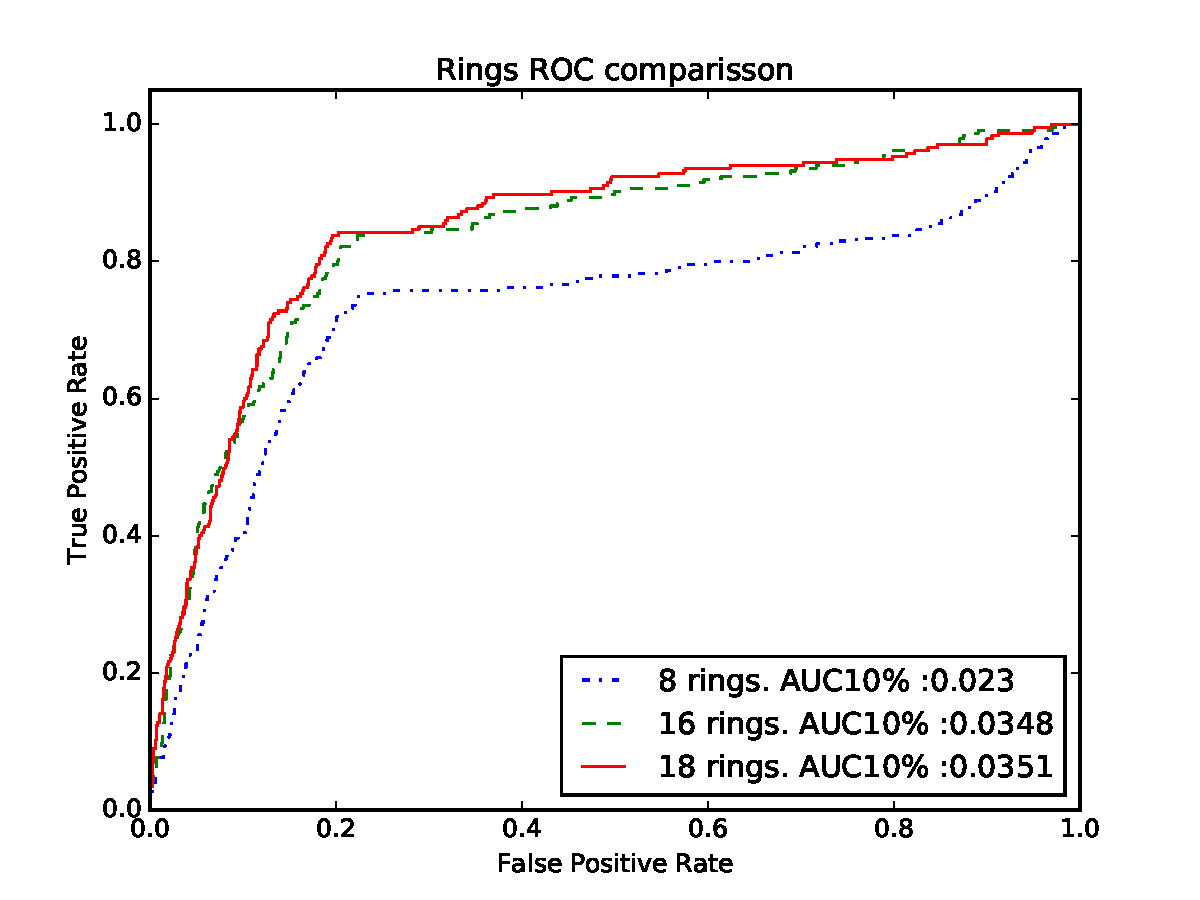
\includegraphics[width=0.8\textwidth]{results/ROC_rings}
\caption{Curvas ROC comparando classificadores SVM sob descritores de anéis com diferentes dimensões.}
\label{fig:roc-rings}
\end{figure}

Tendo visto que o melhor resultado foi obtido com a descrição de 18 dimensões (AUC=0.84), utilizou-se o dataset completo para o treinamento e posterior avaliação através do conjunto de validação, como visto nas tabelas seguintes.

\begin{table}[h!]
\cfmat{Anéis concêntricos com 18 dimensões, dataset completo}{9890}{4}{79}{1143}
\cfmat{Anéis concêntricos com 18 dimensões, conjunto validação}{2564}{174}{158}{77}
\end{table}

\subsection{Classificador profundo}

\subsubsection{MLP}
Na estrutura MLP foram realizados testes com duas e três camadas intermediárias, com ativação RELU e um único perceptron de saída com ativação sigmoide indicando a probabilidade da amostra ser uma cabeça. Essa estrutura da saída como probabilidade é vantajosa pois permite ajustar o compromisso entre falso positivos e falso negativos do classificador, após treinamento, através da escolha do limiar de probabilidade $T$. Escolher um limiar mais alto significa exigir mais segurança do classificador e, portanto, reduzir o número de falsos positivos ao preço de possivelmente aumentar o número de falsos negativos.

Na configuração de duas camadas foram utilizados 512 e 256 perceptrons, respectivamente. Os resultados obtidos para o dataset e conjunto de validação foram os seguintes.
\begin{table}[h!]
\cfmat{MLP 2 camadas, $T=0.5$, dataset completo}{9805}{89}{100}{1122}
\cfmat{MLP 2 camadas, $T=0.9$, dataset completo}{9864}{30}{239}{983}

\cfmat{MLP 2 camadas, $T=0.5$, conjunto validação}{2644}{94}{45}{190}
\cfmat{MLP 2 camadas, $T=0.9$, conjunto validação}{2707}{29}{88}{147}
\end{table}

Para três camadas foram utilizados 1024, 512 e 256 perceptrons respectivamente, entretanto os resultados foram semelhantes aos obtidos com duas camadas, portanto o aumento em complexidade não é justificado visto que o desempenho permaneceu o mesmo.

\subsubsection{Redes convolucionais}
Para redes convolucionais utilizou-se uma única camada convolucional RELU com 16 núcleos 3x3 seguida por max-pooling (3x3) e uma camada densamente conectada de 128 percepetrons RELU e finalmente saída única com ativação sigmoide. Essa topologia foi a que teve o melhor desempenho, obtendo 100\% de acurácia no conjunto de treinamento e 96.97\% no conjunto de validação, como observado a seguir.

\begin{table}[h!]
\cfmat{CNN, $T=0.5$, conjunto de validação}{2660}{78}{23}{212}
\cfmat{CNN, $T=0.9$, conjunto de validação}{2690}{48}{42}{193}
\end{table}

Tendo obtido o melhor desempenho até então, extendeu-se o conjunto de treinamento para 16898 amostras, das quais 14966 são negativas, e o processo de treinamento foi novamente efetuado, obtendo 99.9\% de acurácia no treinamento e 97.54\% no conjunto de validação, como visto a seguir.

\begin{table}[h!]
\cfmat{CNN treinamento extendido, $T=0.5$, conjunto de validação}{2672}{66}{14}{221}
\cfmat{CNN treinamento extendido, $T=0.9$, conjunto de validação}{2686}{52}{21}{214}
\end{table}

Os resultados demonstram que essa topologia de rede é bastante eficiente para o problema em questão. Embora tenha ocorrido um aumento dos falsos positivos de 4 após extender o conjunto de treinamento, isso é justificável pela redução dos falsos negativos, que caiu pela metade, de 42 para 21.

\subsection{Discussão}
Para os diferentes classificadores observou-se as tabelas de confusão correspondentes. Porém essa comparação é facilitada através de um gráfico de curvas ROC dos classificadores correspondentes avaliados no dataset de validação como ilustra a figura \ref{fig:ROC}. Deseja-se obter o melhor classificador, isto é, o classificador com maior AUC. 

Observa-se que muitos classificadores obtiveram um desempenho elevado no conjunto de treinamento, em especial as redes convolucionais que obtiveram acurácia unitária (sob dataset balanceado), demonstrando a alta capacidade do modelo. Nota-se, entretanto, que há grande discrepância entre o desempenho dos classificadores no conjunto de treinamento e de validação, o que caracteriza \textit{overfitting}, e fica mais evidenciado nos métodos superficiais. Os métodos profundos, em contraste, apresentam uma boa generalização. Isso é explicado porque o modelo em questão foi corretamente especificado através no número de camadas e tamanho de filtros, de forma que sua capacidade se ajuste de forma adequada aos dados.

\begin{figure}[ht]
\centering
\begin{subfigure}{.5\textwidth}
  \centering
  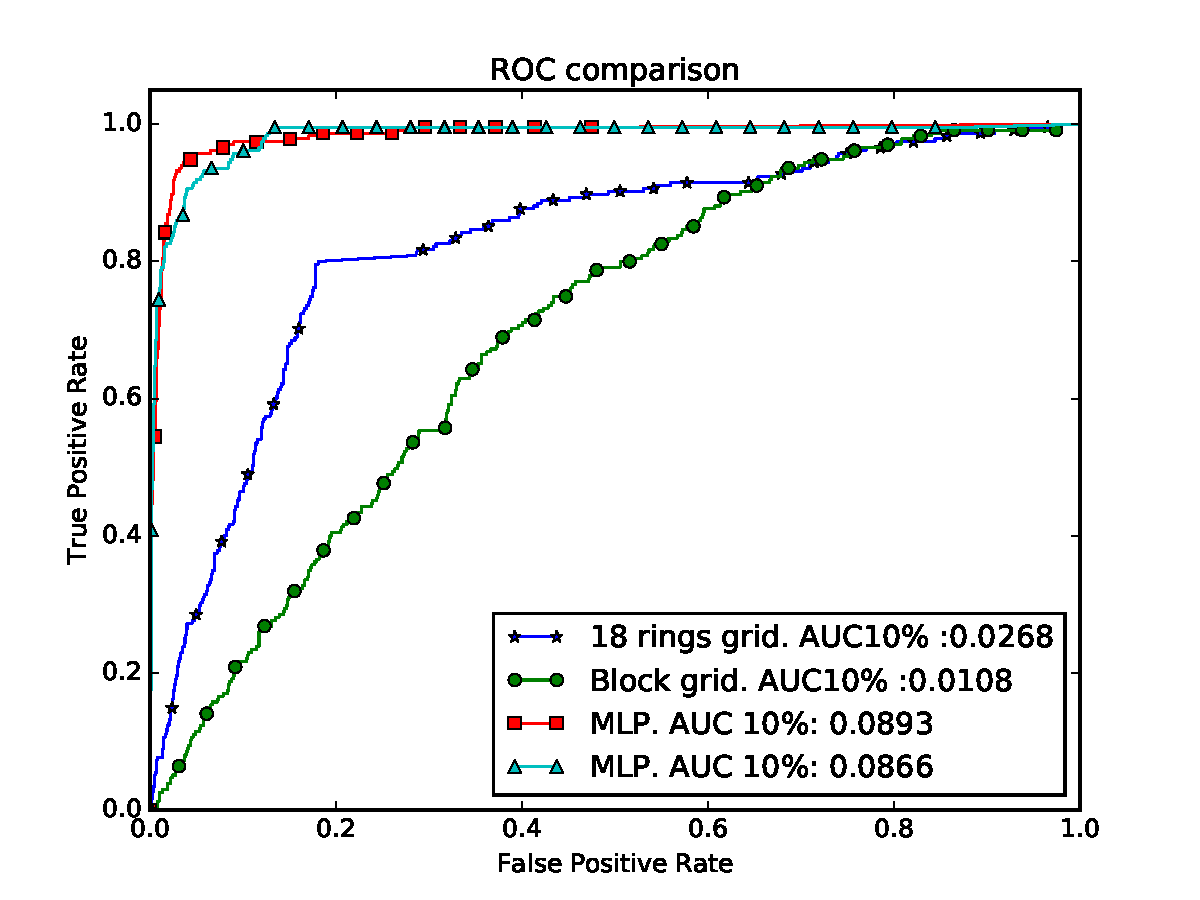
\includegraphics[width=\linewidth]{results/ROC_all}
\end{subfigure}%
\begin{subfigure}{.5\textwidth}
  \centering
  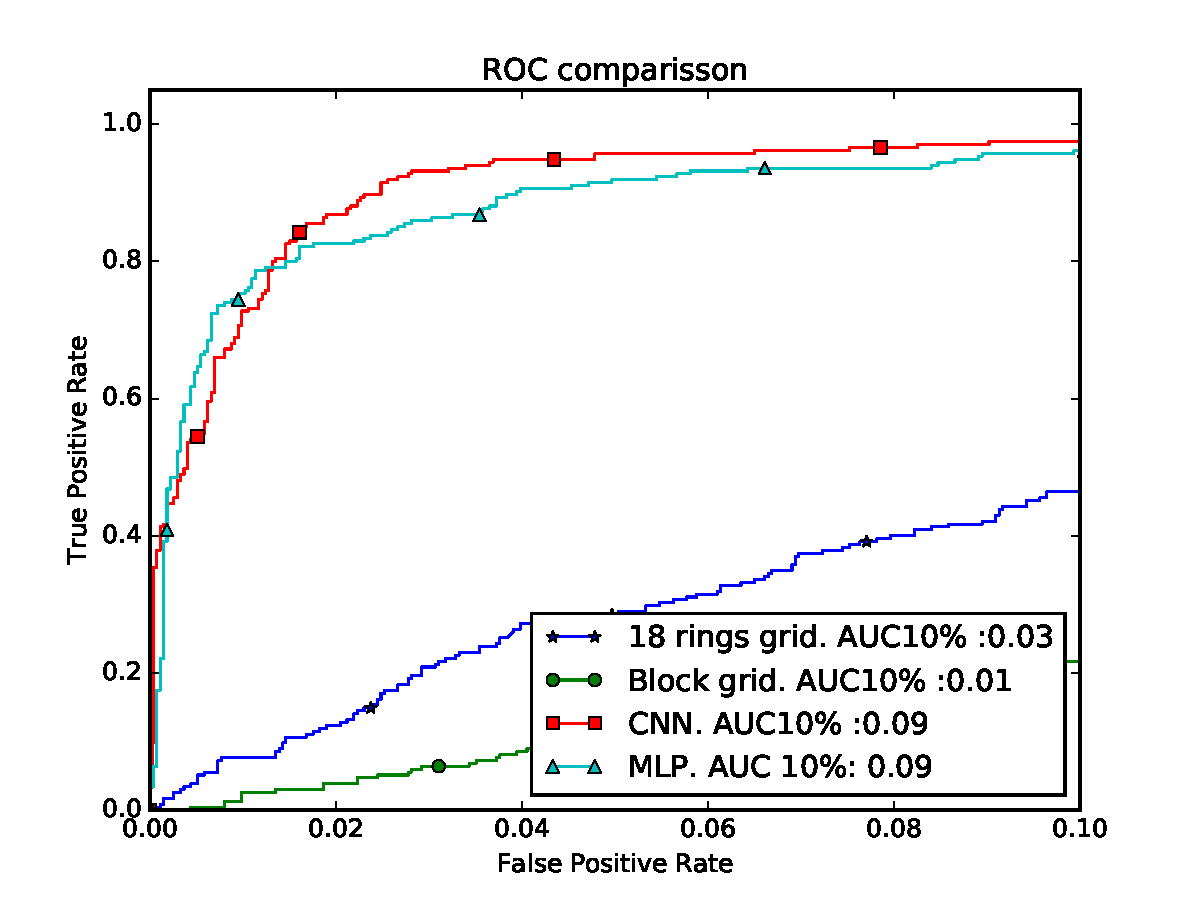
\includegraphics[width=\linewidth]{results/ROC_all_zoom}
\end{subfigure}
\caption{Curvas ROC comparativa dos diferentes classificadores apresentados e zoom na região de interesse}
\label{fig:ROC}
\end{figure}

Conclui-se, então, que a melhor solução para classificação é a rede convolucional, oferencendo um bom compromisso entre TVP e TFP para a aplicação em questão, onde é mais importante que os falsos positivos sejam minimizados para evitar paralisação frequente da produção. Além disso, é possível utilizar a imagem da direita em \ref{fig:ROC}, que representa a região de operação tradicional (baixo TFP), para selecionar um limiar de probabilidade $T$ para garantir que TFP não ultrapasse um limite especificado, ao preço de diminuir a TVP.

\section{Sistema completo}
Nessa seção serão comparados os resultados do sistema de extração de candidatos e de classificação como um todo. Tendo em vista os resultados da seção \ref{sec:resultados-classificadores}, a solução baseada na seleção de candidatos vista em \ref{sec:tradicional-candidatos} e classificador CNN apresentada no capítulo \ref{chap:class-profundo} será avaliada em detrimento das demais variações de classificadores. A última solução, cuja detecção e classificação são realizadas utilizando métodos profundos, vista no capítulo X também será avaliada.
